\section{Molecular Dynamics at a Desired Temperature}

\subsection*{Programming}

For the \emph{velocity rescaling} thermostat we can derive the rescaling-factor $\fr$ from equation \eqref{6fr1}.
\begin{align}
\frac{3}{2}k_BT_0
	&= \frac{\Ekino}{N}
	\label{6fr1}\\
&= \frac{1}{N}\sum_{i=1}^{N} \frac{(\fr\cdot\vecv{i})^2}{2m}
	\label{6fr2}\\
&= \fr^2\frac{\Ekin}{N}
	\label{6fr3}\\
&=\fr^2\frac{3}{2}k_BT
	\label{6fr4}\\
\fr
	&= \sqrt{\frac{T_0}{T}}
	\label{6r5}
\end{align}

This rescaling is implemented in C. In fact the implementation in C is not much faster than in python, but the thermostat in python did some crazy stuff.
The function c\_velocity\_rescaling can be seen in code block \ref{6rescaling}.

\listfile[MyCstyle]{../src/c_lj.cpp}{src/c\_lj.cpp}{281}{286}{Velocity rescaling}{6rescaling}

This function is used in the main loop in ljsim.py every time after meausuring the observalbles.\\

To start the thermostat you can use the command line option \ls{--tstat} which accepts the desired temperature as argument (see code block \ref{comsim}).
The option \ls{--ctstat} is there for continuing the simulation for the interrupted simulation with temperature T thermostat, but now with deactivated thermostat.
This is necessary because the programm saves the results of the simulation with different names for different temperatures.

\subsection*{Measurement}

\begin{figure}[ht]

Obs.
\hfill
\begin{subfigure}{0.3\textwidth}
\centering
$T_0 = 0.3$
\end{subfigure}
\hfill
\begin{subfigure}{0.3\textwidth}
\centering
$T_0 = 1.0$
\end{subfigure}
\hfill
\begin{subfigure}{0.3\textwidth}
\centering
$T_0 = 2.0$
\end{subfigure}

T
\hfill
\begin{subfigure}{0.3\textwidth}
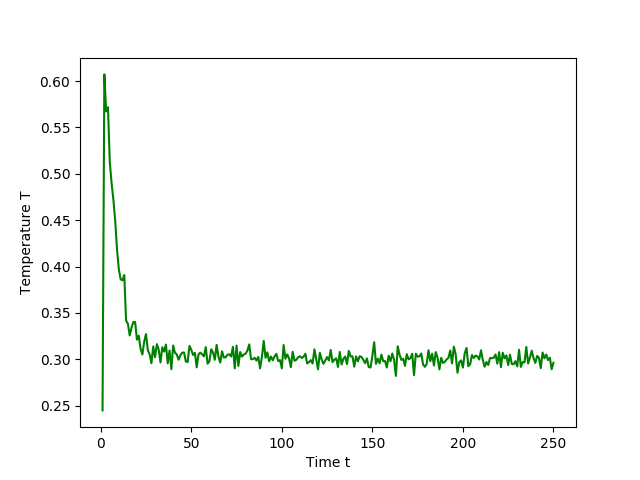
\includegraphics[width=\textwidth]{../dat/Temperature_T0d3.png}
\end{subfigure}
\hfill
\begin{subfigure}{0.3\textwidth}
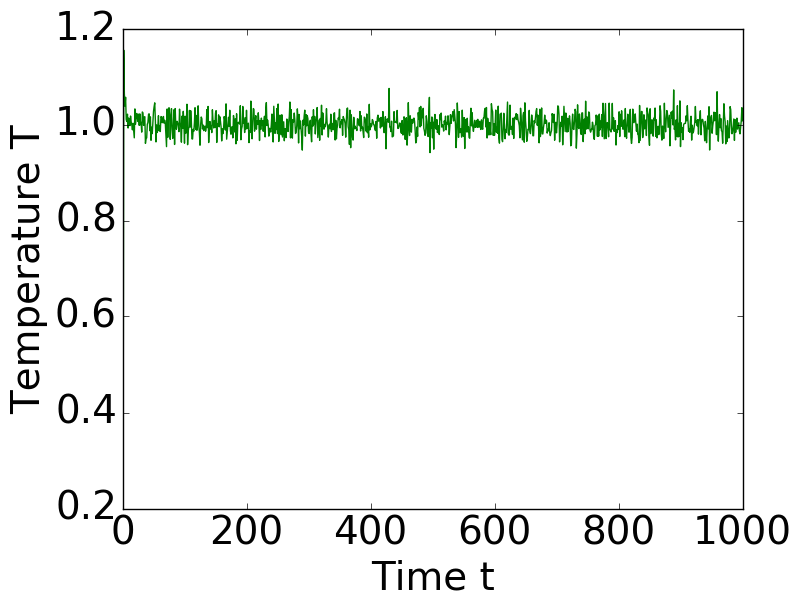
\includegraphics[width=\textwidth]{../dat/Temperature_T1d0.png}
\end{subfigure}
\hfill
\begin{subfigure}{0.3\textwidth}
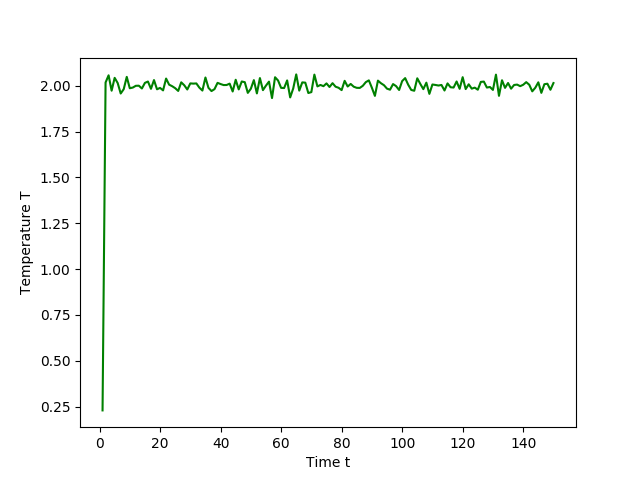
\includegraphics[width=\textwidth]{../dat/Temperature_T2d0.png}
\end{subfigure}

E
\hfill
\begin{subfigure}{0.3\textwidth}
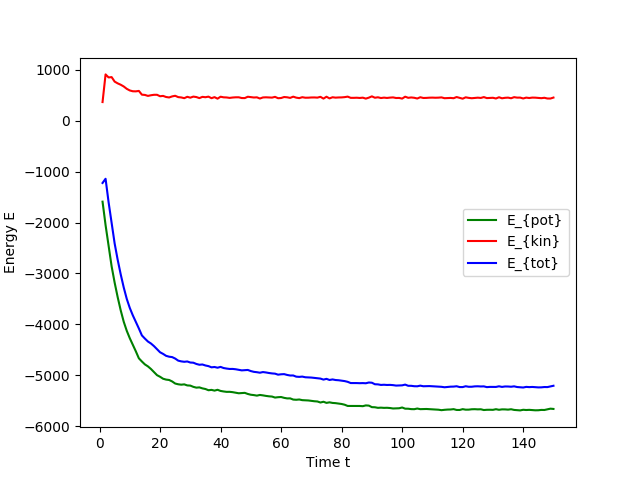
\includegraphics[width=\textwidth]{../dat/Energies_T0d3.png}
\end{subfigure}
\hfill
\begin{subfigure}{0.3\textwidth}
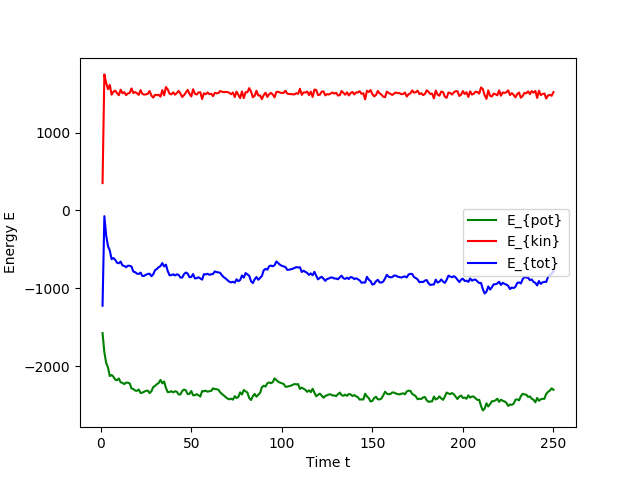
\includegraphics[width=\textwidth]{../dat/Energies_T1d0.png}
\end{subfigure}
\hfill
\begin{subfigure}{0.3\textwidth}
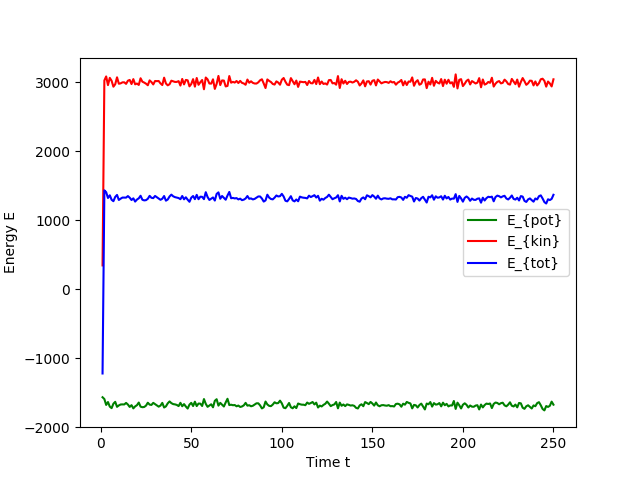
\includegraphics[width=\textwidth]{../dat/Energies_T2d0.png}
\end{subfigure}

U
\hfill
\begin{subfigure}{0.3\textwidth}
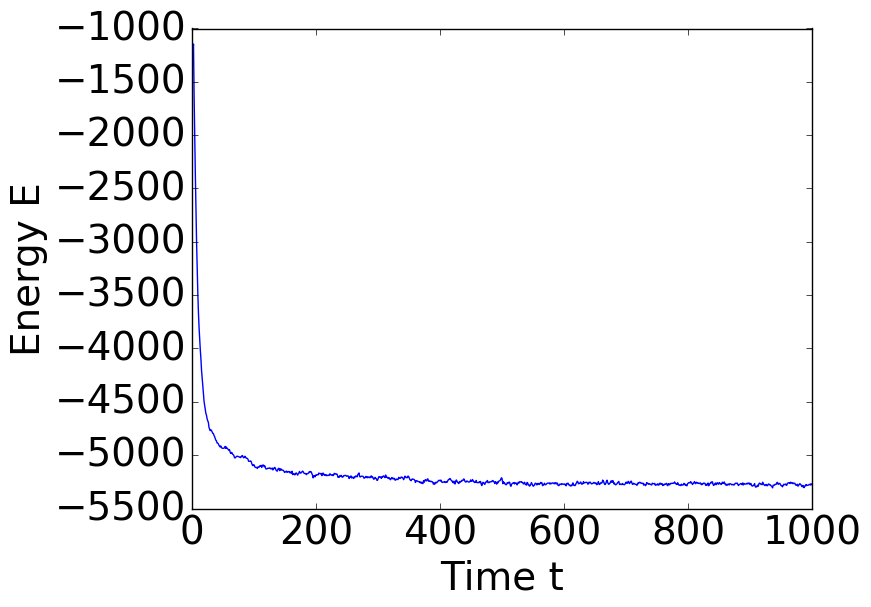
\includegraphics[width=\textwidth]{../dat/Total_Energy_T0d3.png}
\end{subfigure}
\hfill
\begin{subfigure}{0.3\textwidth}
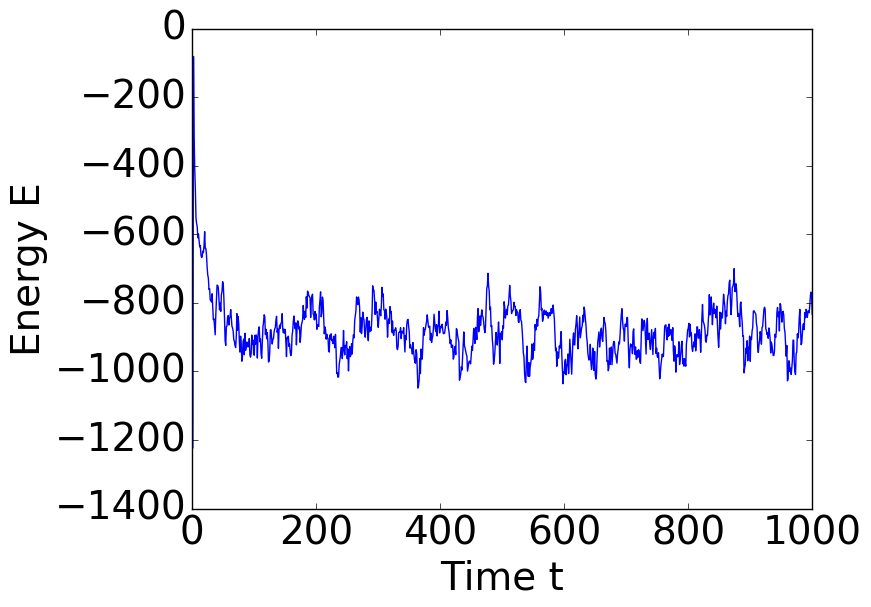
\includegraphics[width=\textwidth]{../dat/Total_Energy_T1d0.png}
\end{subfigure}
\hfill
\begin{subfigure}{0.3\textwidth}
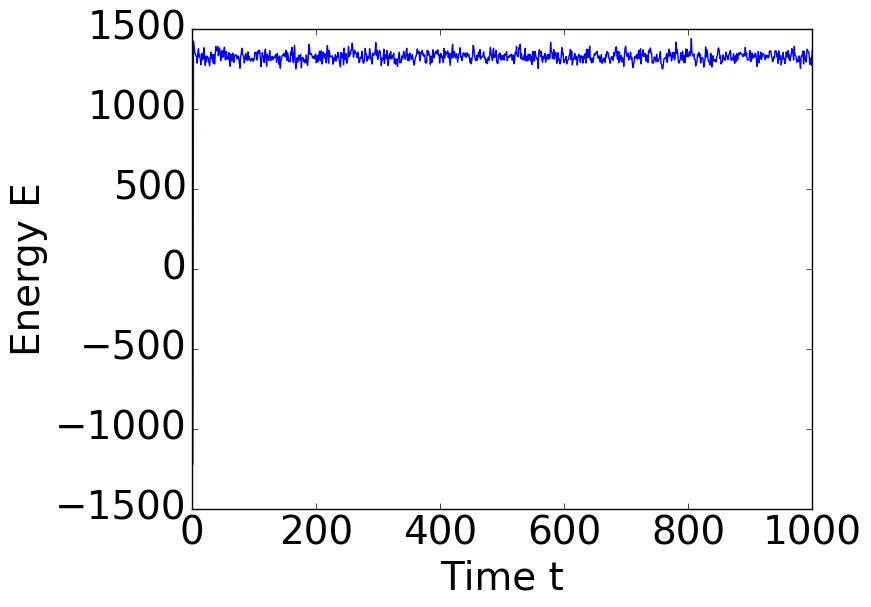
\includegraphics[width=\textwidth]{../dat/Total_Energy_T2d0.png}
\end{subfigure}

P
\hfill
\begin{subfigure}{0.3\textwidth}
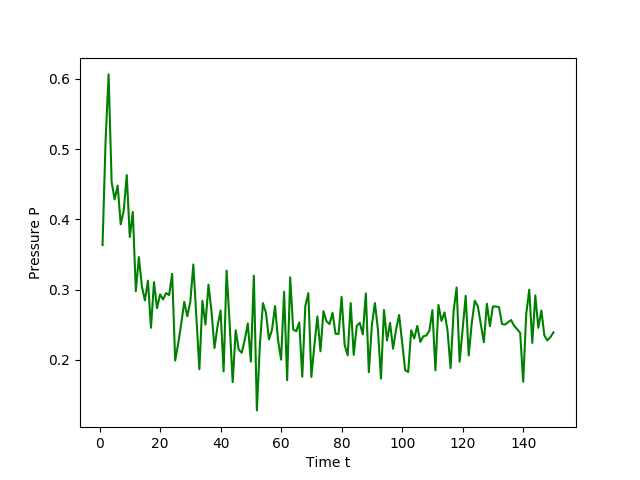
\includegraphics[width=\textwidth]{../dat/Pressure_T0d3.png}
\end{subfigure}
\hfill
\begin{subfigure}{0.3\textwidth}
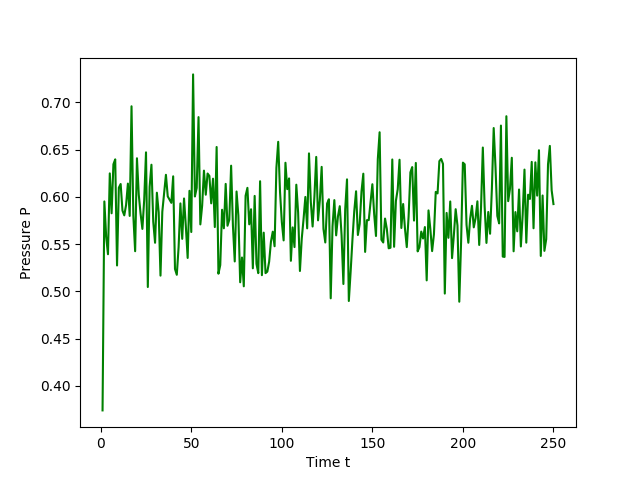
\includegraphics[width=\textwidth]{../dat/Pressure_T1d0.png}
\end{subfigure}
\hfill
\begin{subfigure}{0.3\textwidth}
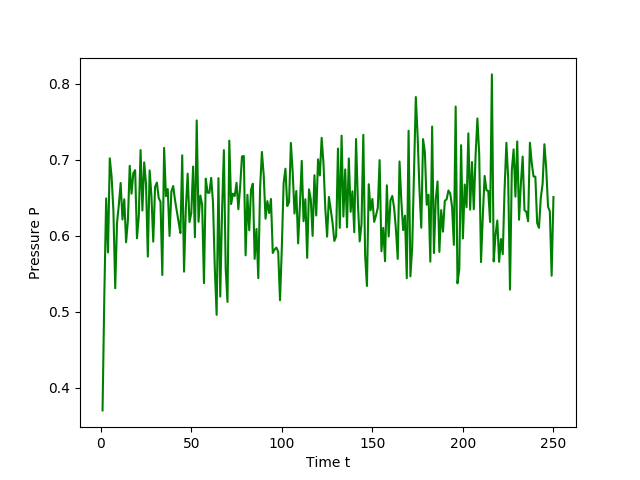
\includegraphics[width=\textwidth]{../dat/Pressure_T2d0.png}
\end{subfigure}

\caption{
Measured Observables (Obs.) for a thermostat temperature $T_O$.\\
T is the real temperature of the system, E are the energies (green: potential, red: kinetic, blue: total).\\
U is the total energy of the system alone.\\
P is the pressure of the system.}
\label{fig4}
\end{figure}


Now we can test the simulation for desired temperatures of  $T_0\epsilon\left\lbrace 0.3,1.0,2.0\right\rbrace $. Figure \ref{fig4} shows the results for a time period of t=150.\\

As you can see the equilibration time seems to be highest for $T_O=0.3$ and lowest for $T_O=2.0$. 
This is because the temperature $T_0=0.3$ is much lower than the initial temperature. 
Therefor the total energy of the system must decrease. But the positive kinetic energy is much lower, than the necessary energy differece. 
If the temperature should be $T=0.3$ the potential energy of the system must decrease, but it is not directly effected by the velocity rescaling.
By contrast for $T_0=2.0$ the necessary energy can simply  be reached by increasing the kinetic energy because it is much higher than the initial energy.\\

For $T_0=1.0$ the necessary energy is not much different from the initial one and therefor the other effects on equilibration have a higher influence.